\icode{N21Q-EME-SI-L3-261121-001}
\nceeID[3]{2021海南}{8}
如图，\(V\)型对接的绝缘斜面\(M\)、\(N\)固定在水平面上，两斜面与水平面夹角均为\(\alpha =\) \,\qty{60}{\degree}，其中斜面\(N\)光滑。两个质量相同的带电小滑块\(P\)、\(Q\)分别静止在\(M\)、\(N\)上，\(P\)、\(Q\)连线垂直于斜面\(M\)，已知最大静摩擦力等于滑动摩擦力。则\(P\)与\(M\)间的动摩擦因数至少\paren[]

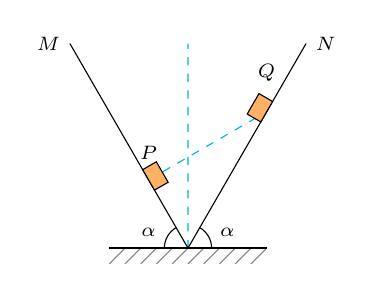
\begin{tikzpicture}[>=stealth,font=\scriptsize]
	\draw[dashed,cyan] (120:1)--(60:2) (0,0)--(0,{1.5*sqrt(3)});
	\draw[rotate=-60] (0,0)--(-3,0)node[left]{\(M\)};
	\draw[fill=orange!60,rotate=-60] (-.85,0) rectangle(-1.15,.2);
	\draw[rotate=60] (0,0)--(3,0)node[right]{\(N\)};
	\draw[fill=orange!60,rotate=60] (1.85,0) rectangle(2.15,.2);
	\foreach \x in {-1,-.8,...,.8}
		\draw[gray] (\x,-.2)--++(.2,.2);
	\draw[thick] (-1,0)--(1,0);
	\draw (-.3,0) arc(180:120:.3);
	\draw (.3,0) arc(0:60:.3);
	\node at(-.5,1)[above]{\(P\)};
	\node at(1,2)[above]{\(Q\)};
	\node at(-.5,.2){\(\alpha\)};
	\node at(.5,.2){\(\alpha\)};
\end{tikzpicture}
\begin{choices}
	\item \(\sfrac{\sqrt{3}}{6}\)
	\item \(\sfrac{1}{2}\)
	\item \(\sfrac{\sqrt{3}}{2}\)
	\item \(\sfrac{\sqrt{3}}{3}\)
\end{choices}
\begin{answer}
	
\end{answer}